\subsection{Self-Supervision under Severe Missingness}
\label{sec:exp-missingness-regime}

The benefit of self-supervision depends on how much the encoder is starved of features. To make this precise, we compare NESS (with its hist and path objectives) against the no-SSL baseline as the missing rate increases from $0.8$ to $0.95$ on ogbn-arxiv. Figure~\ref{fig:missingness} shows the result. Both configurations degrade as features become scarcer, but the no-SSL baseline degrades faster, so the advantage of self-supervision widens: the gain over no-SSL grows from $+0.005$ at $\rho=0.8$ to $+0.031$ at $\rho=0.95$. When observed features are abundant the encoder already recovers most of the signal and self-supervision adds little; as the graph becomes information-starved, the self-supervised objectives contribute an increasingly large share of the usable signal. This is the regime in which self-supervision is most valuable.

\begin{figure}[t]
\centering
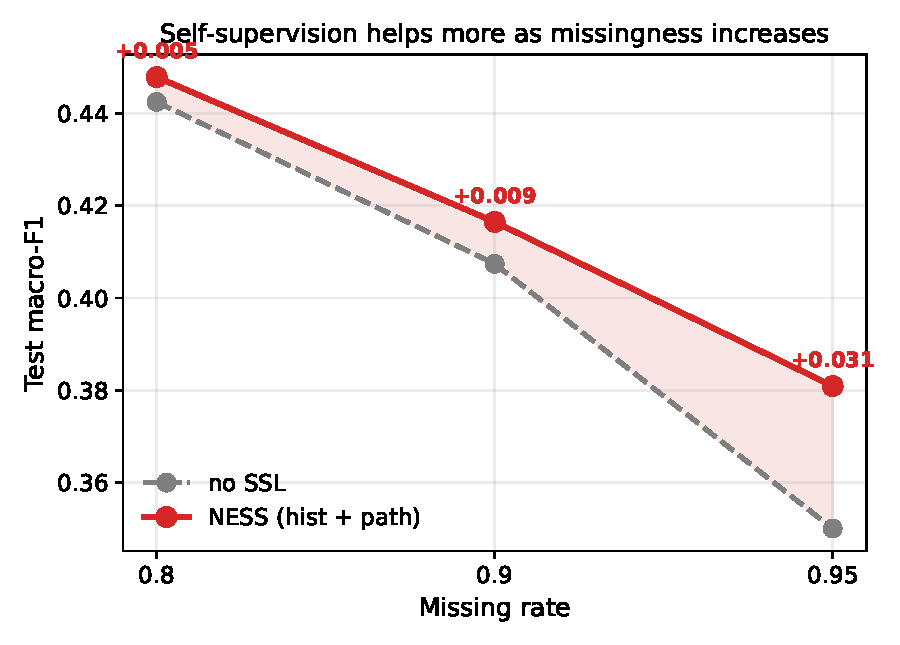
\includegraphics[width=0.85\linewidth]{figures/e12_missingness.pdf}
\caption{Test macro-F1 on ogbn-arxiv as the missing rate increases. Both NESS (hist + path) and the no-SSL baseline decline, but the self-supervised model declines more slowly; the gap (shaded) grows from $+0.005$ at $80\%$ missing to $+0.031$ at $95\%$.}
\label{fig:missingness}
\end{figure}
